
For the model hyperbolic problem 
\begin{equation}
\dfrac{\dr u}{\dr t}+a\dfrac{\dr u}{\dr x}=0
\end{equation}
with $a>0$, $0<x<2$ and $t>0$. We consider the initial condition $u(x,0)=0$ for $0<x\leq 2$. Since $a>0$ the solution will travel towards the right and we need a boundary condition on the left-hand side of the domain. Take the square signal 
$$
u(0,t)=\left\{\begin{array}{lcc}
1 & -(n+1)T/2<t\leq -nT/2 & n = 0,2,4\dots\\
-1 & -(n+1)T/2<t\leq -nT/2 & n = 1,3,5\dots
\end{array}\right.
$$
where $T$ is the period time.

The point of interest is to compare the behaviour of three methods 1) upwind, 2) Lax-Friedrich
and 3) Lax-Wendroff. lets first define the following methods.

\paragraph*{1) Upwind FTBS} The upwind method uses forward time and backward space schemes. So we get the first order in space and time 
$$u_{i,k+1}=(1-\sigma)u_{i,k}+\sigma u_{i-1,k}.$$ 


\paragraph*{2) Lax-Friedrich method} is defined by 
$$u_{i,k+1} = \dfrac{u_{i-1,k}+u_{i+1,k}}{2}-\dfrac{\sigma}{2}(u_{i+1,k}-u_{i-1,k}).$$

\paragraph*{3) Lax-Wendroff method} is defined by 
$$u_{i,k+1} = u_{i,k} -\dfrac{\sigma}{2}(u_{i+1,k}-u_{i-1,k}) +\dfrac{\sigma^2}{2}(u_{i+1,k}-2u_{i,k}+u_{i-1,k}).$$


We look at the results on the test problem for the values $\sigma = \{0.8, 1, 1.1\}$. It is clear on figure~\ref{fig:1} that $\sigma=1.1$ gives an unstable scheme for each method. And the "magic" $\sigma=1$ transports the solution as it should. The interesting points to analyse are in the case $\sigma=0.8$ where different behaviour occur. The upwind and Lax-Friedrich methods introduce a smoothing. This is an illustration of an artificial dissipation\red{possibilité d'ajouter l'équation modifiée}. Finally, the Lax-Wendroff generates oscillations, this is to be expected for a method that is second order in time and the errors come from the dispersion in the numerical method.\red{cool mais je ne comprend pas trop ce que ça veut dire, c'est page 16 des notes} 

\begin{figure}[!h]
\centering
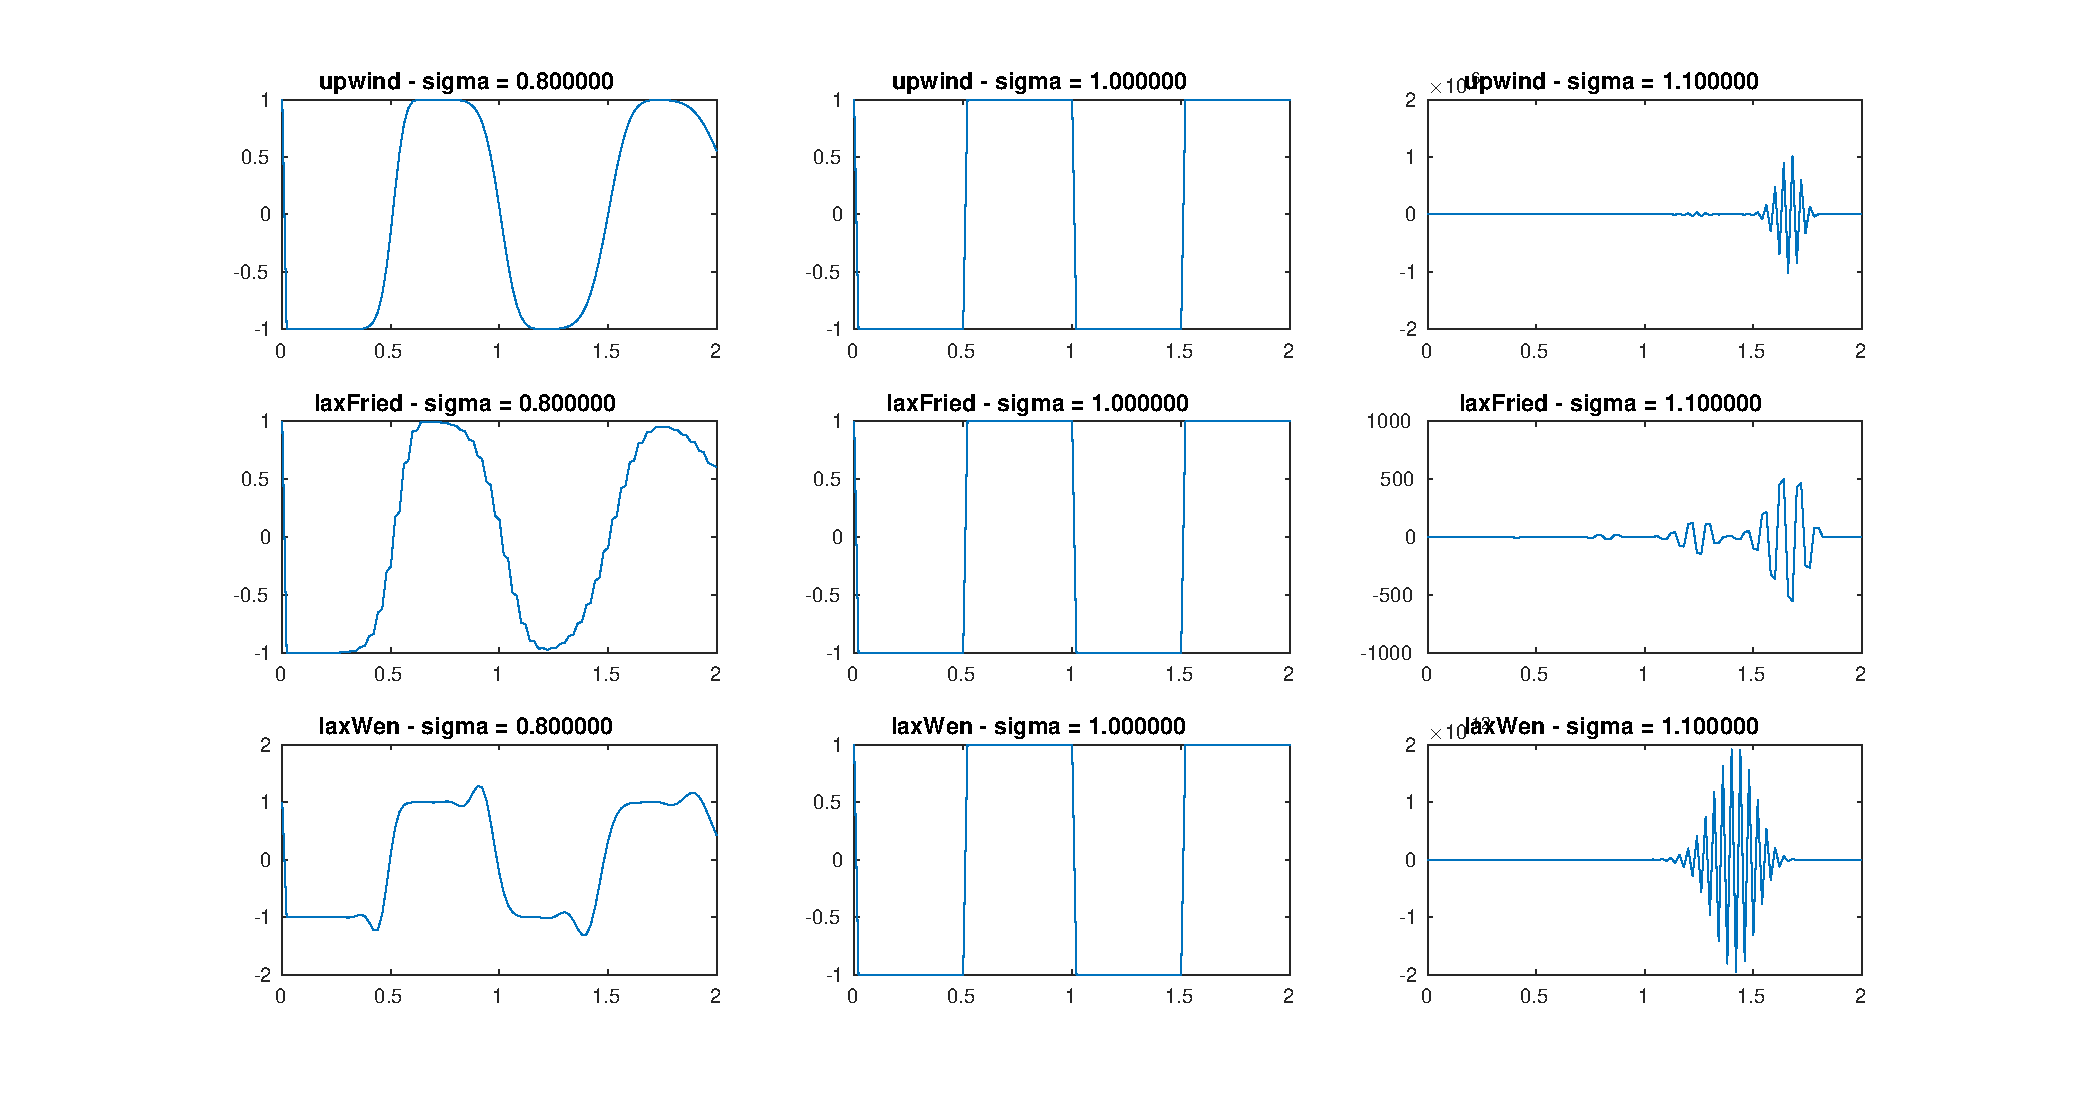
\includegraphics[scale = 0.5]{./fig1.eps}
\caption{Results for the different methods}
\label{fig:1}
\end{figure}
